        %%******************************************%%
        %%                                          %%
        %%        Modello di tesi di laurea         %%
        %%            di Andrea Giraldin            %%
        %%                                          %%
        %%             2 novembre 2012              %%
        %%                                          %%
        %%******************************************%%


% I seguenti commenti speciali impostano:
% 1. 
% 2. PDFLaTeX come motore di composizione;
% 3. tesi.tex come documento principale;
% 4. il controllo ortografico italiano per l'editor.

% !TEX encoding = UTF-8
% !TEX TS-program = pdflatex
% !TEX root = tesi.tex
% !TEX spellcheck = it-IT

\documentclass[10pt,                    % corpo del font principale
               a4paper,                 % carta A4
               twoside,                 % impagina per fronte-retro
               openright,               % inizio capitoli a destra
               english,                 
               italian,                 
               ]{book}    

%**************************************************************
% Importazione package
%************************************************************** 

%\usepackage{amsmath,amssymb,amsthm}    % matematica

\usepackage{longtable}

\usepackage[T1]{fontenc}                % codifica dei font:
                                        % NOTA BENE! richiede una distribuzione *completa* di LaTeX

\usepackage[utf8]{inputenc}             % codifica di input; anche [latin1] va bene
                                        % NOTA BENE! va accordata con le preferenze dell'editor

\usepackage[english, italian]{babel}    % per scrivere in italiano e in inglese;
                                        % l'ultima lingua (l'italiano) risulta predefinita

\usepackage{bookmark}                   % segnalibri

\usepackage{caption}                    % didascalie

\usepackage{chngpage,calc}              % centra il frontespizio

\usepackage{csquotes}                   % gestisce automaticamente i caratteri (")

\usepackage{emptypage}                  % pagine vuote senza testatina e piede di pagina

\usepackage{epigraph}			% per epigrafi

\usepackage{eurosym}                    % simbolo dell'euro

%\usepackage{indentfirst}               % rientra il primo paragrafo di ogni sezione

\usepackage{graphicx}                   % immagini

\usepackage{newunicodechar}             % problemi con alcuni caratteri
\newunicodechar{fi}{fi}
\newunicodechar{ff}{ff}

\usepackage{hyperref}                   % collegamenti ipertestuali

\usepackage[binding=5mm]{layaureo}      % margini ottimizzati per l'A4; rilegatura di 5 mm

\usepackage{listings}                   % codici

\usepackage{microtype}                  % microtipografia

\usepackage{mparhack,fixltx2e,relsize}  % finezze tipografiche

\usepackage{nameref}                    % visualizza nome dei riferimenti                                      

\usepackage[font=small]{quoting}        % citazioni

\usepackage{subfig}                     % sottofigure, sottotabelle

\usepackage[italian]{varioref}          % riferimenti completi della pagina

\usepackage[dvipsnames]{xcolor}         % colori

\usepackage{booktabs}                   % tabelle                                       
\usepackage{tabularx}                   % tabelle di larghezza prefissata                                    
\usepackage{longtable}                  % tabelle su più pagine                                        
\usepackage{ltxtable}                   % tabelle su più pagine e adattabili in larghezza

\usepackage[toc, acronym]{glossaries}   % glossario
                                        % per includerlo nel documento bisogna:
                                        % 1. compilare una prima volta tesi.tex;
                                        % 2. eseguire: makeindex -s tesi.ist -t tesi.glg -o tesi.gls tesi.glo
                                        % 3. eseguire: makeindex -s tesi.ist -t tesi.alg -o tesi.acr tesi.acn
                                        % 4. compilare due volte tesi.tex.

\usepackage[backend=biber,style=verbose-ibid,hyperref,backref]{biblatex}
                                        % eccellente pacchetto per la bibliografia; 
                                        % produce uno stile di citazione autore-anno; 
                                        % lo stile "numeric-comp" produce riferimenti numerici
                                        % per includerlo nel documento bisogna:
                                        % 1. compilare una prima volta tesi.tex;
                                        % 2. eseguire: biber tesi
                                        % 3. compilare ancora tesi.tex.

%**************************************************************
% file contenente le impostazioni della tesi
%**************************************************************

%**************************************************************
% Frontespizio
%**************************************************************

% Comando per il nome dell'azienda

\newcommand{\visione}{VisioneImpresa}

% Contatore dei paragrafi

\setcounter{secnumdepth}{4}

% comando per i termini di Glossario

\newcommand{\glossaryItem}[1]{%
    \lowercase{\ifcsname @glsterms@\detokenize{#1}\endcsname}%
        #1%
    \else%
        \lowercase{\expandafter\gdef\csname @glsterms@\detokenize{#1}\endcsname{x}}%
        \emph{#1}\ped{G}%
    \fi%
}

% Comando per nuovo paragrafo

\newcommand{\myparagraph}[1]{\paragraph{#1}\mbox{} \mbox{}}


% Autore
\newcommand{\myName}{Tommaso Carraro}                                    
\newcommand{\myTitle}{Titolo della tesi}

% Tipo di tesi                   
\newcommand{\myDegree}{Tesi di laurea triennale}

% Università             
\newcommand{\myUni}{Università degli Studi di Padova}

% Facoltà       
\newcommand{\myFaculty}{Corso di Laurea in Informatica}

% Dipartimento
\newcommand{\myDepartment}{Dipartimento di Matematica "Tullio Levi-Civita"}

% Titolo del relatore
\newcommand{\profTitle}{Prof.}

% Relatore
\newcommand{\myProf}{Armir Bujari}

% Luogo
\newcommand{\myLocation}{Padova}

% Anno accademico
\newcommand{\myAA}{2017-2018}

% Data discussione
\newcommand{\myTime}{Dicembre 2018}


%**************************************************************
% Impostazioni di impaginazione
% see: http://wwwcdf.pd.infn.it/AppuntiLinux/a2547.htm
%**************************************************************

\setlength{\parindent}{14pt}   % larghezza rientro della prima riga
\setlength{\parskip}{0pt}   % distanza tra i paragrafi


%**************************************************************
% Impostazioni di biblatex
%**************************************************************
\bibliography{bibliografia} % database di biblatex 

\defbibheading{bibliography} {
    \cleardoublepage
    \phantomsection 
    \addcontentsline{toc}{chapter}{\bibname}
    \chapter*{\bibname\markboth{\bibname}{\bibname}}
}

\setlength\bibitemsep{1.5\itemsep} % spazio tra entry

\DeclareBibliographyCategory{opere}
\DeclareBibliographyCategory{web}

\addtocategory{opere}{womak:lean-thinking}
\addtocategory{web}{site:agile-manifesto}

\defbibheading{opere}{\section*{Riferimenti bibliografici}}
\defbibheading{web}{\section*{Siti Web consultati}}


%**************************************************************
% Impostazioni di caption
%**************************************************************
\captionsetup{
    tableposition=top,
    figureposition=bottom,
    font=small,
    format=hang,
    labelfont=bf
}

%**************************************************************
% Impostazioni di glossaries
%**************************************************************

%**************************************************************
% Acronimi
%**************************************************************
\renewcommand{\acronymname}{Acronimi e abbreviazioni}

\newacronym[description={\glslink{apig}{Application Program Interface}}]
    {api}{API}{Application Program Interface}

\newacronym[description={\glslink{umlg}{Unified Modeling Language}}]
    {uml}{UML}{Unified Modeling Language}

%**************************************************************
% Glossario
%**************************************************************
%\renewcommand{\glossaryname}{Glossario}

\newglossaryentry{apig}
{
    name=\glslink{api}{API},
    text=Application Program Interface,
    sort=api,
    description={in informatica con il termine \emph{Application Programming Interface API} (ing. interfaccia di programmazione di un'applicazione) si indica ogni insieme di procedure disponibili al programmatore, di solito raggruppate a formare un set di strumenti specifici per l'espletamento di un determinato compito all'interno di un certo programma. La finalità è ottenere un'astrazione, di solito tra l'hardware e il programmatore o tra software a basso e quello ad alto livello semplificando così il lavoro di programmazione}
}

\newglossaryentry{umlg}
{
    name=\glslink{uml}{UML},
    text=UML,
    sort=uml,
    description={in ingegneria del software \emph{UML, Unified Modeling Language} (ing. linguaggio di modellazione unificato) è un linguaggio di modellazione e specifica basato sul paradigma object-oriented. L'\emph{UML} svolge un'importantissima funzione di ``lingua franca'' nella comunità della progettazione e programmazione a oggetti. Gran parte della letteratura di settore usa tale linguaggio per descrivere soluzioni analitiche e progettuali in modo sintetico e comprensibile a un vasto pubblico}
}
 % database di termini
\makeglossaries


%**************************************************************
% Impostazioni di graphicx
%**************************************************************
\graphicspath{{immagini/}} % cartella dove sono riposte le immagini


%**************************************************************
% Impostazioni di hyperref
%**************************************************************
\hypersetup{
    %hyperfootnotes=false,
    %pdfpagelabels,
    %draft,	% = elimina tutti i link (utile per stampe in bianco e nero)
    colorlinks=true,
    linktocpage=true,
    pdfstartpage=1,
    pdfstartview=FitV,
    % decommenta la riga seguente per avere link in nero (per esempio per la stampa in bianco e nero)
    %colorlinks=false, linktocpage=false, pdfborder={0 0 0}, pdfstartpage=1, pdfstartview=FitV,
    breaklinks=true,
    pdfpagemode=UseNone,
    pageanchor=true,
    pdfpagemode=UseOutlines,
    plainpages=false,
    bookmarksnumbered,
    bookmarksopen=true,
    bookmarksopenlevel=1,
    hypertexnames=true,
    pdfhighlight=/O,
    %nesting=true,
    %frenchlinks,
    urlcolor=webbrown,
    linkcolor=RoyalBlue,
    citecolor=webgreen,
    %pagecolor=RoyalBlue,
    %urlcolor=Black, linkcolor=Black, citecolor=Black, %pagecolor=Black,
    pdftitle={\myTitle},
    pdfauthor={\textcopyright\ \myName, \myUni, \myFaculty},
    pdfsubject={},
    pdfkeywords={},
    pdfcreator={pdfLaTeX},
    pdfproducer={LaTeX}
}

%**************************************************************
% Impostazioni di itemize
%**************************************************************
\renewcommand{\labelitemi}{$\ast$}

%\renewcommand{\labelitemi}{$\bullet$}
%\renewcommand{\labelitemii}{$\cdot$}
%\renewcommand{\labelitemiii}{$\diamond$}
%\renewcommand{\labelitemiv}{$\ast$}


%**************************************************************
% Impostazioni di listings
%**************************************************************
\lstset{
    language=[LaTeX]Tex,%C++,
    keywordstyle=\color{RoyalBlue}, %\bfseries,
    basicstyle=\small\ttfamily,
    %identifierstyle=\color{NavyBlue},
    commentstyle=\color{Green}\ttfamily,
    stringstyle=\rmfamily,
    numbers=none, %left,%
    numberstyle=\scriptsize, %\tiny
    stepnumber=5,
    numbersep=8pt,
    showstringspaces=false,
    breaklines=true,
    frameround=ftff,
    frame=single
} 


%**************************************************************
% Impostazioni di xcolor
%**************************************************************
\definecolor{webgreen}{rgb}{0,.5,0}
\definecolor{webbrown}{rgb}{.6,0,0}


%**************************************************************
% Altro
%**************************************************************

\newcommand{\omissis}{[\dots\negthinspace]} % produce [...]

% eccezioni all'algoritmo di sillabazione
\hyphenation
{
    ma-cro-istru-zio-ne
    gi-ral-din
}

\newcommand{\sectionname}{sezione}
\addto\captionsitalian{\renewcommand{\figurename}{Figura}
                       \renewcommand{\tablename}{Tabella}}

\newcommand{\glsfirstoccur}{\ap{{[g]}}}

\newcommand{\intro}[1]{\emph{\textsf{#1}}}

%**************************************************************
% Environment per ``rischi''
%**************************************************************
\newcounter{riskcounter}                % define a counter
\setcounter{riskcounter}{0}             % set the counter to some initial value

%%%% Parameters
% #1: Title
\newenvironment{risk}[1]{
    \refstepcounter{riskcounter}        % increment counter
    \par \noindent                      % start new paragraph
    \textbf{\arabic{riskcounter}. #1}   % display the title before the 
                                        % content of the environment is displayed 
}{
    \par\medskip
}

\newcommand{\riskname}{Rischio}

\newcommand{\riskdescription}[1]{\textbf{\\Descrizione:} #1.}

\newcommand{\risksolution}[1]{\textbf{\\Soluzione:} #1.}

%**************************************************************
% Environment per ``use case''
%**************************************************************
\newcounter{usecasecounter}             % define a counter
\setcounter{usecasecounter}{0}          % set the counter to some initial value

%%%% Parameters
% #1: ID
% #2: Nome
\newenvironment{usecase}[2]{
    \renewcommand{\theusecasecounter}{\usecasename #1}  % this is where the display of 
                                                        % the counter is overwritten/modified
    \refstepcounter{usecasecounter}             % increment counter
    \vspace{10pt}
    \par \noindent                              % start new paragraph
    {\large \textbf{\usecasename #1: #2}}       % display the title before the 
                                                % content of the environment is displayed 
    \medskip
}{
    \medskip
}

\newcommand{\usecasename}{UC}

\newcommand{\usecaseactors}[1]{\textbf{\\Attori Principali:} #1. \vspace{4pt}}
\newcommand{\usecasepre}[1]{\textbf{\\Precondizioni:} #1. \vspace{4pt}}
\newcommand{\usecasedesc}[1]{\textbf{\\Descrizione:} #1. \vspace{4pt}}
\newcommand{\usecasepost}[1]{\textbf{\\Postcondizioni:} #1. \vspace{4pt}}
\newcommand{\usecasealt}[1]{\textbf{\\Scenario Alternativo:} #1. \vspace{4pt}}

%**************************************************************
% Environment per ``namespace description''
%**************************************************************

\newenvironment{namespacedesc}{
    \vspace{10pt}
    \par \noindent                              % start new paragraph
    \begin{description} 
}{
    \end{description}
    \medskip
}

\newcommand{\classdesc}[2]{\item[\textbf{#1:}] #2}                     % file con le impostazioni personali

\begin{document}
%**************************************************************
% Materiale iniziale
%**************************************************************
\frontmatter
% !TEX encoding = UTF-8
% !TEX TS-program = pdflatex
% !TEX root = ../tesi.tex

%**************************************************************
% Frontespizio 
%**************************************************************
\begin{titlepage}

\begin{center}

\begin{LARGE}
\textbf{\myUni}\\
\end{LARGE}

\vspace{10pt}

\begin{Large}
\textsc{\myDepartment}\\
\end{Large}

\vspace{10pt}

\begin{large}
\textsc{\myFaculty}\\
\end{large}

\vspace{30pt}
\begin{figure}[htbp]
\begin{center}

\includegraphics[height=6cm]{logo-unipd}
\end{center}
\end{figure}
\vspace{30pt} 

\begin{LARGE}
\begin{center}
\textbf{\myTitle}\\
\end{center}
\end{LARGE}

\vspace{10pt} 

\begin{large}
\textsl{\myDegree}\\
\end{large}

\vspace{40pt} 

\begin{large}
\begin{flushleft}
\textit{Relatore}\\ 
\vspace{5pt} 
\profTitle \myProf
\end{flushleft}

\vspace{0pt} 

\begin{flushright}
\textit{Laureando}\\ 
\vspace{5pt} 
\myName
\end{flushright}
\end{large}

\vspace{40pt}

\line(1, 0){338} \\
\begin{normalsize}
\textsc{Anno Accademico \myAA}
\end{normalsize}

\end{center}
\end{titlepage} 
% !TEX encoding = UTF-8
% !TEX TS-program = pdflatex
% !TEX root = ../tesi.tex

%**************************************************************
% Colophon
%**************************************************************
\clearpage
\phantomsection
\thispagestyle{empty}

\hfill

\vfill

\noindent\myName: \textit{\myTitle,}
\myDegree,
\textcopyright\ \myTime.
% !TEX encoding = UTF-8
% !TEX TS-program = pdflatex
% !TEX root = ../tesi.tex

%**************************************************************
% Dedica
%**************************************************************
\cleardoublepage
\phantomsection
\thispagestyle{empty}
\pdfbookmark{Dedica}{Dedica}

\vspace*{3cm}

\begin{center}
Lorem ipsum dolor sit amet, consectetuer adipiscing elit. \\ \medskip
--- Oscar Wilde    
\end{center}

\medskip

\begin{center}
Dedicato a ...
\end{center}

% !TEX encoding = UTF-8
% !TEX TS-program = pdflatex
% !TEX root = ../tesi.tex

%**************************************************************
% Sommario
%**************************************************************
\cleardoublepage
\phantomsection
\pdfbookmark{Sommario}{Sommario}
\begingroup
\let\clearpage\relax
\let\cleardoublepage\relax
\let\cleardoublepage\relax

\chapter*{Sommario}

Il presente documento descrive il lavoro svolto durante il periodo di \textit{stage}, della durata di 320 ore, dal laureando Tommaso Carraro presso l'azienda \visione{} S.r.l. situata a Pernumia (PD).

Lo scopo principale del progetto era la realizzazione di un'applicazione \textit{mobile} che permettesse ai clienti di una qualsiasi azienda di acquistare, tramite il proprio \textit{smartphone}, dei prodotti venduti dalla stessa. Per raggiungere questo fine sono stati assegnati vari compiti.

Lo studente ha dovuto scegliere in autonomia l'ambiente di sviluppo ritenuto più opportuno. Poiché era richiesto che l'applicazione funzionasse sia in ambiente \textit{Android} che in ambiente \textit{iOS}, si è dovuto scegliere un \glossaryItem{framework cross-platfrom} e, in particolare, il \glossaryItem{framework} \textit{PhoneGap}.

In seguito alla scelta del \textit{framework} vi è stato un periodo di formazione, di circa 40 ore, sui \textit{software} gestionali utilizzati in azienda e sul linguaggio \textit{JavaScript}, in modo da facilitare lo sviluppo del progetto.

Si è poi potuto proseguire con la progettazione delle varie componenti della \glossaryItem{piattaforma}, quali \glossaryItem{servizio web}, \textit{database} sottostanti, logica applicativa e interfaccia grafica. 
L'applicazione doveva funzionare interamente \textit{online}, nessun dato doveva essere memorizzato in locale, per cui il servizio \textit{web} e i \textit{database} sono stati installati su un \textit{server} \glossaryItem{Azure} di proprietà dell'azienda.
In particolare, è stato richiesto di progettare un \textit{database} che permettesse la gestione dei dati di autenticazione e un \textit{database} che contenesse i dati utili alla gestione degli ordini presso un'azienda cliente. Il \textit{database} contenente i dati proprietari dell'azienda poteva essere locale al \textit{server Azure} o all'interno di un \textit{server cloud} dell'azienda stessa, a seconda delle scelte effettuate da quest'ultima.

In seguito alla progettazione delle varie parti si è iniziata l'implementazione della piattaforma. Il servizio doveva gestire le richieste \glossaryItem{HTTP} (\textit{HyperText Transfer Protocol}) provenienti dall'applicazione tramite oggetti \glossaryItem{servlet} \textit{Java} e rispondere a queste mediante stringhe in formato \glossaryItem{JSON}.
La logica applicativa dell'applicazione doveva essere scritta in linguaggio \textit{JavaScript}, questo perché lo stagista ha scelto il \textit{framework PhoneGap}. Per permettere all'applicazione di comunicare con il servizio \textit{web} tramite richieste \textit{HTTP}, si è dovuta utilizzare la tecnica \glossaryItem{AJAX} (\textit{Asynchronous JavaScript And XML}).
Il \textit{design} dell'interfaccia doveva essere simile al \textit{design} di un'altra applicazione sviluppata dall'azienda, chiamata \glossaryItem{moviDOC}. Infine, per permettere all'applicazione di essere \glossaryItem{usabile} dalla maggior parte dei dispositivi, si è dovuto rendere il \textit{design} della stessa \glossaryItem{responsive}.

%\vfill
%
%\selectlanguage{english}
%\pdfbookmark{Abstract}{Abstract}
%\chapter*{Abstract}
%
%\selectlanguage{italian}

\endgroup			

\vfill


% !TEX encoding = UTF-8
% !TEX TS-program = pdflatex
% !TEX root = ../tesi.tex

%**************************************************************
% Ringraziamenti
%**************************************************************
\cleardoublepage
\phantomsection
\pdfbookmark{Ringraziamenti}{ringraziamenti}

\begin{flushright}{
	\slshape    
	``Life is really simple, but we insist on making it complicated''} \\ 
	\medskip
    --- Confucius
\end{flushright}


\bigskip

\begingroup
\let\clearpage\relax
\let\cleardoublepage\relax
\let\cleardoublepage\relax

\chapter*{Ringraziamenti}

\noindent \textit{Innanzitutto, vorrei esprimere la mia gratitudine al Dott. Armir Bujari, relatore della mia tesi, per l'aiuto e il sostegno fornitomi durante la stesura del lavoro e per avermi ricevuto nel suo ufficio ogniqualvolta gli è stato possibile.}\\

\noindent \textit{Ringrazio il mio tutor aziendale, Francesco Turra, per avermi dato la possibilità di lavorare a \visione{}, ma soprattutto per avermi assegnato un progetto a cui ero interessato. Non lo ringrazierò mai abbastanza per avermi concesso di lavorare da casa alcuni giorni mentre preparavo un esame importante, e per avermi aiutato ad ottenere la borsa di studio ``Mille e una lode'', prolungando di un mese il periodo di stage.}\\

\noindent \textit{Merita di essere nominato il mio collega Luca, sviluppatore di \visione{}, senza l'aiuto del quale non avrei terminato il progetto nei tempi prestabiliti. La sua esperienza mi ha permesso di risolvere gran parte dei problemi riscontrati durante lo sviluppo del progetto.}\\

\noindent \textit{Desidero ringraziare con affetto mia madre Federica, mio padre Gianni e mio fratello Edoardo, per il sostegno e il grande aiuto ricevuti durante questi anni di studio, ma soprattutto per la grande pazienza dimostrata nei periodi più impegnativi di questo terzo anno, durante il quale non sono sempre stato presente.}\\

\noindent \textit{Ringrazio infinitamente il Professor Tullio Vardanega per avermi aiutato ad ottenere la borsa di studio ``Mille e una lode'' e per aver risposto tempestivamente a tutte le mail concernenti l'argomento.}\\

\noindent \textit{Ringrazio il mio collega universitario Alberto per avermi aiutato a preparare tutti gli esami durante questi anni di studio a Padova.}\\

\noindent \textit{Ringrazio i miei cari amici Margherita e Gabriele per essermi sempre stati accanto e per il conforto ricevuto durante i momenti cupi della mia vita.}\\

\noindent \textit{Ho desiderio di ringraziare poi la ``BMX family'', che alimenta ogni giorno la passione che covo per questo bellissimo sport e stile di vita.}\\

\noindent \textit{Ringrazio infine Elisa, la ragazza che ho amato e con la quale ho passato i momenti più belli di questo 2018.}
\bigskip

\noindent\textit{\myLocation{}, 10 \myTime{}}
\hfill \myName

\endgroup


% !TEX encoding = UTF-8
% !TEX TS-program = pdflatex
% !TEX root = ../tesi.tex

%**************************************************************
% Indici
%**************************************************************
\cleardoublepage
\pdfbookmark{\contentsname}{tableofcontents}
\setcounter{tocdepth}{2}
\tableofcontents
%\markboth{\contentsname}{\contentsname} 
\clearpage

\begingroup 
    \let\clearpage\relax
    \let\cleardoublepage\relax
    \let\cleardoublepage\relax
    %*******************************************************
    % Elenco delle figure
    %*******************************************************    
    \phantomsection
    \pdfbookmark{\listfigurename}{lof}
    \listoffigures

    \vspace*{8ex}

    %*******************************************************
    % Elenco delle tabelle
    %*******************************************************
    \phantomsection
    \pdfbookmark{\listtablename}{lot}
    \listoftables
        
    \vspace*{8ex}
\endgroup

\cleardoublepage

\cleardoublepage

%**************************************************************
% Materiale principale
%**************************************************************
\mainmatter
% !TEX encoding = UTF-8
% !TEX TS-program = pdflatex
% !TEX root = ../tesi.tex

%**************************************************************
\chapter{Introduzione}
\label{cap:introduzione}
%**************************************************************

Introduzione al contesto applicativo.\\

\noindent Esempio di utilizzo di un termine nel glossario \\
\gls{api}. \\

\noindent Esempio di citazione in linea \\
\cite{site:agile-manifesto}. \\

\noindent Esempio di citazione nel pie' di pagina \\
citazione\footcite{womak:lean-thinking} \\

%**************************************************************
\section{L'azienda}

Descrizione dell'azienda.

%**************************************************************
\section{L'idea}

Introduzione all'idea dello stage.

%**************************************************************
\section{Organizzazione del testo}

\begin{description}
    \item[{\hyperref[cap:processi-metodologie]{Il secondo capitolo}}] descrive ...
    
    \item[{\hyperref[cap:descrizione-stage]{Il terzo capitolo}}] approfondisce ...
    
    \item[{\hyperref[cap:analisi-requisiti]{Il quarto capitolo}}] approfondisce ...
    
    \item[{\hyperref[cap:progettazione-codifica]{Il quinto capitolo}}] approfondisce ...
    
    \item[{\hyperref[cap:verifica-validazione]{Il sesto capitolo}}] approfondisce ...
    
    \item[{\hyperref[cap:conclusioni]{Nel settimo capitolo}}] descrive ...
\end{description}

Riguardo la stesura del testo, relativamente al documento sono state adottate le seguenti convenzioni tipografiche:
\begin{itemize}
	\item gli acronimi, le abbreviazioni e i termini ambigui o di uso non comune menzionati vengono definiti nel glossario, situato alla fine del presente documento;
	\item per la prima occorrenza dei termini riportati nel glossario viene utilizzata la seguente nomenclatura: \emph{parola}\glsfirstoccur;
	\item i termini in lingua straniera o facenti parti del gergo tecnico sono evidenziati con il carattere \emph{corsivo}.
\end{itemize}             % Introduzione
% !TEX encoding = UTF-8
% !TEX TS-program = pdflatex
% !TEX root = ../tesi.tex

%**************************************************************
\chapter{Processi e metodologie}
\label{cap:processi-metodologie}
%**************************************************************

\intro{Brevissima introduzione al capitolo}\\

%**************************************************************
\section{Processo sviluppo prodotto}             % Processi
% !TEX encoding = UTF-8
% !TEX TS-program = pdflatex
% !TEX root = ../tesi.tex

%**************************************************************
\chapter{Descrizione dello stage}
\label{cap:descrizione-stage}
%**************************************************************

\intro{Breve introduzione al capitolo}\\

%**************************************************************
\section{Introduzione al progetto}

%**************************************************************
\section{Analisi preventiva dei rischi}

Durante la fase di analisi iniziale sono stati individuati alcuni possibili rischi a cui si potrà andare incontro.
Si è quindi proceduto a elaborare delle possibili soluzioni per far fronte a tali rischi.\\

\begin{risk}{Performance del simulatore hardware}
    \riskdescription{le performance del simulatore hardware e la comunicazione con questo potrebbero risultare lenti o non abbastanza buoni da causare il fallimento dei test}
    \risksolution{coinvolgimento del responsabile a capo del progetto relativo il simulatore hardware}
    \label{risk:hardware-simulator} 
\end{risk}

%**************************************************************
\section{Requisiti e obiettivi}


%**************************************************************
\section{Pianificazione}             % Kick-Off
% !TEX encoding = UTF-8
% !TEX TS-program = pdflatex
% !TEX root = ../tesi.tex

%**************************************************************
\chapter{Analisi dei requisiti}
\label{cap:analisi-requisiti}
%**************************************************************

Questo capitolo descrive i casi d'uso e i requisiti della piattaforma moviORDER, individuati e classificati per definire nel dettaglio obiettivi e funzionalità del sistema. I casi d'uso e i requisiti sono stati dedotti da un'analisi preliminare eseguita dal tutor aziendale, la quale è stata perfezionata dallo stagista per perseguire massima efficienza ed efficacia del sistema. Le convenzioni adottate per la stesura di casi d'uso e requisiti sono presenti in Appendice §\ref{}.

\section{Casi d'uso}

Per lo studio dei casi di utilizzo della piattaforma sono stati creati dei diagrammi dei casi d'uso che meglio descrivono funzioni e/o servizi offerti dal sistema, così come sono percepiti e utilizzati dagli attori che interagiscono con il sistema stesso. Per la definizione dei diagrammi UML dei casi d'uso è stato utilizzato lo standard UML 2.0.

\subsection{Attori del sistema}

Lo scopo di moviORDER è permettere alle aziende che forniscono dei prodotti di vendere gli stessi ai propri clienti tramite un'applicazione multipiattaforma. Quindi moviORDER viene distribuita da VISIONEIMPRESA alle aziende che forniscono prodotti, la quale viene distribuita dalle aziende stesse ai propri clienti. Gli utilizzatori finali di moviORDER sono quindi i clienti delle singole aziende che sono clienti di VISIONEIMPRESA.
L'accesso all'applicazione è consentito solamente agli utenti provvisti di credenziali di accesso, le quali vengono distribuite, insieme all'applicazione, dal fornitore. Non è prevista quindi una funzionalità di registrazione. Nel contesto di moviORDER vi sono quindi due tipologie di attori:
\begin{enumerate}
	\item \textbf{Utente non autenticato}: è un utente che non ha effettuato l'accesso al sistema al quale viene offerta la sola funzionalità di autenticazione. Una volta che un utente non autenticato viene riconosciuto accedendo al sistema, diventa un utente autenticato;
	\item \textbf{Utente autenticato}: è un utente che ha effettuato l'accesso al sistema e che può usufruire di tutte le sue funzionalità. Le funzionalità offerte all'utente autenticato sono:
	\begin{itemize}
		\item possibilità di effettuare il logout;
		\item possibilità di aggiungere articoli al proprio carrello;
		\item possibilità di modificare gli articoli nel proprio carrello;
		\item possibilità di rimuovere articoli dal proprio carrello;
		\item possibilità di inviare un ordine alla propria azienda.
	\end{itemize}
\end{enumerate}

\subsection{UC1 - Azioni utente non autenticato}

\begin{figure}[!h] 
    \centering 
    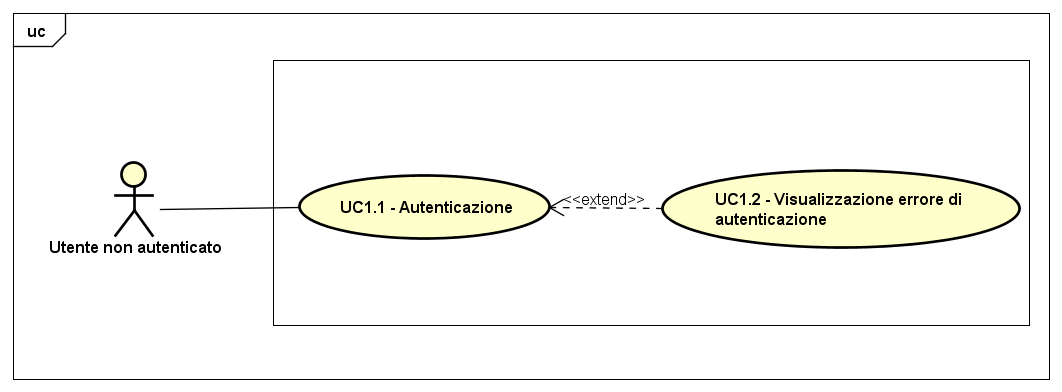
\includegraphics[width=0.9\columnwidth]{usecase/generaleNonAutenticato} 
    \caption{Use Case - UC1: Azioni utente non autenticato}
\end{figure}

\begin{itemize}
	\item \textbf{Attore}: Utente non autenticato;
	\item \textbf{Descrizione}: L'attore può eseguire l'operazione di autenticazione alla piattaforma moviORDER;
	\item \textbf{Pre-condizioni}: L'attore ha avviato l'applicazione, possiede le credenziali di accesso e non è ancora stato riconosciuto dal sistema;
	\item \textbf{Post-condizioni}: L'attore ha eseguito l'operazione di autenticazione;
	\item \textbf{Scenario principale}: UC1.1 - Autenticazione;
	\item \textbf{Scenario alternativo}: L'attore ha fornito credenziali di accesso non corrispondenti a nessun utente registrato dall'azienda, oppure non riesce ad accedere al sistema perché è stato bloccato dall'azienda stessa: UC1.2 - Visualizzazione errore di autenticazione. 
\end{itemize}

\subsection{UC1.1 - Autenticazione}

\begin{figure}[!h] 
    \centering 
    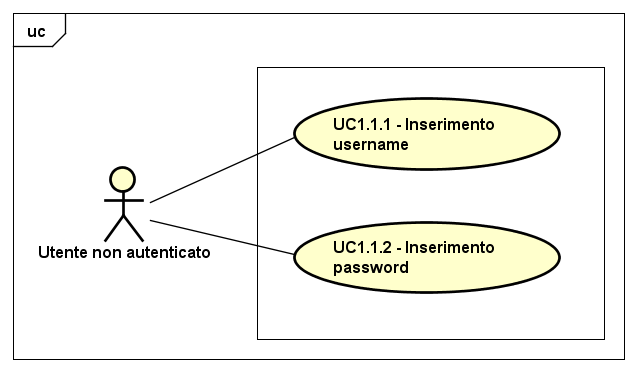
\includegraphics[width=0.9\columnwidth]{usecase/autenticazione} 
    \caption{Use Case - UC1.1: Autenticazione}
\end{figure}

\begin{itemize}
	\item \textbf{Attore}: Utente non autenticato;
	\item \textbf{Descrizione}: L'attore può eseguire l'operazione di autenticazione;
	\item \textbf{Pre-condizioni}: L’attore ha avviato l’applicazione, non è ancora riconosciuto dal sistema ed ha espresso la volontà di effettuare l’autenticazione a moviORDER;
	\item \textbf{Post-condizioni}: L’attore ha eseguito l’operazione di accesso al sistema ed è quindi ora riconosciuto come utente autenticato;
	\item \textbf{Scenario principale}: 
		\begin{enumerate}
			\item UC1.1.1 - Inserimento username;
			\item UC1.1.2 - Inserimento password.
		\end{enumerate} 
\end{itemize}

\subsection{UC2 - Azioni utente autenticato}

\begin{figure}[!h] 
    \centering 
    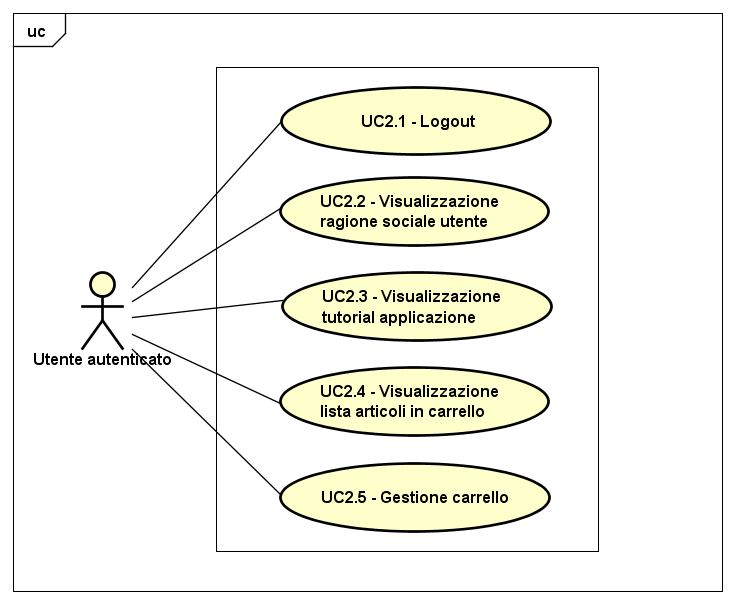
\includegraphics[width=0.9\columnwidth]{usecase/generaleAutenticato} 
    \caption{UC2 - Azioni utente autenticato}
    \label{fig:altoLivello2}
\end{figure}

\begin{itemize}
	\item \textbf{Attore}: Utente autenticato;
	\item \textbf{Descrizione}: L'attore può:
	\begin{enumerate}
		\item Eseguire l'operazione di logout;
		\item Visualizzare la propria ragione sociale;
		\item Visualizzare il tutorial dell'applicazione premendo sul relativo bottone;
		\item Visualizzare la lista degli articoli in carrello;
		\item Gestire il proprio carrello. 
	\end{enumerate}
	\item \textbf{Pre-condizioni}: L'attore è stato riconosciuto dal sistema;
	\item \textbf{Post-condizioni}: L'attore ha eseguito le azioni che desiderava compiere all'interno del sistema;
	\item \textbf{Scenario principale}: 
		\begin{enumerate}
			\item UC2.1 - Logout;
			\item UC2.2 - Visualizzazione ragione sociale utente;
			\item UC2.3 - Visualizzazione tutorial applicazione;
			\item UC2.4 - Visualizzazione lista articoli in carrello;
			\item UC2.5 - Gestione carrello.
		\end{enumerate}
\end{itemize}

\subsection{UC2.4 - Visualizzazione lista articoli in carrello}

\subsection{UC2.4.1 - Visualizzazione singolo articolo in carrello}

\subsection{UC2.5 - Gestione carrello}

\subsection{UC2.5.1 - Aggiunta articolo}

\subsection{UC2.5.2 - Modifica articolo}

\subsection{UC2.5.11 - Invio ordine}

\section{Tracciamento dei requisiti}

Da un'attenta analisi dei requisiti e degli use case effettuata sul progetto è stata stilata la tabella che traccia i requisiti in rapporto agli use case.\\
Sono stati individuati diversi tipi di requisiti e si è quindi fatto utilizzo di un codice identificativo per distinguerli.\\
Il codice dei requisiti è così strutturato R(F/Q/V)(N/D/O) dove:
\begin{enumerate}
	\item[R =] requisito
    \item[F =] funzionale
    \item[Q =] qualitativo
    \item[V =] di vincolo
    \item[N =] obbligatorio (necessario)
    \item[D =] desiderabile
    \item[Z =] opzionale
\end{enumerate}
Nelle tabelle \ref{tab:requisiti-funzionali}, \ref{tab:requisiti-qualitativi} e \ref{tab:requisiti-vincolo} sono riassunti i requisiti e il loro tracciamento con gli use case delineati in fase di analisi.

\newpage

\begin{table}%
\caption{Tabella del tracciamento dei requisti funzionali}
\label{tab:requisiti-funzionali}
\begin{tabularx}{\textwidth}{lXl}
\hline\hline
\textbf{Requisito} & \textbf{Descrizione} & \textbf{Use Case}\\
\hline
RFN-1     & L'interfaccia permette di configurare il tipo di sonde del test & UC1 \\
\hline
\end{tabularx}
\end{table}%

\begin{table}%
\caption{Tabella del tracciamento dei requisiti qualitativi}
\label{tab:requisiti-qualitativi}
\begin{tabularx}{\textwidth}{lXl}
\hline\hline
\textbf{Requisito} & \textbf{Descrizione} & \textbf{Use Case}\\
\hline
RQD-1    & Le prestazioni del simulatore hardware deve garantire la giusta esecuzione dei test e non la generazione di falsi negativi & - \\
\hline
\end{tabularx}
\end{table}%

\begin{table}%
\caption{Tabella del tracciamento dei requisiti di vincolo}
\label{tab:requisiti-vincolo}
\begin{tabularx}{\textwidth}{lXl}
\hline\hline
\textbf{Requisito} & \textbf{Descrizione} & \textbf{Use Case}\\
\hline
RVO-1    & La libreria per l'esecuzione dei test automatici deve essere riutilizzabile & - \\
\hline
\end{tabularx}
\end{table}%             % Concept Preview
% !TEX encoding = UTF-8
% !TEX TS-program = pdflatex
% !TEX root = ../tesi.tex

%**************************************************************
\chapter{Progettazione e codifica}
\label{cap:progettazione-codifica}
%**************************************************************

\intro{Breve introduzione al capitolo}\\

%**************************************************************
\section{Tecnologie e strumenti}
\label{sec:tecnologie-strumenti}

Di seguito viene data una panoramica delle tecnologie e strumenti utilizzati.

\subsection*{Tecnologia 1}
Descrizione Tecnologia 1.

\subsection*{Tecnologia 2}
Descrizione Tecnologia 2

%**************************************************************
\section{Ciclo di vita del software}
\label{sec:ciclo-vita-software}

%**************************************************************
\section{Progettazione}
\label{sec:progettazione}

\subsubsection{Namespace 1} %**************************
Descrizione namespace 1.

\begin{namespacedesc}
    \classdesc{Classe 1}{Descrizione classe 1}
    \classdesc{Classe 2}{Descrizione classe 2}
\end{namespacedesc}


%**************************************************************
\section{Design Pattern utilizzati}

%**************************************************************
\section{Codifica}
             % Product Prototype
% !TEX encoding = UTF-8
% !TEX TS-program = pdflatex
% !TEX root = ../tesi.tex

%**************************************************************
\chapter{Verifica e validazione}
\label{cap:verifica-validazione}
%**************************************************************             % Product Design Freeze e SOP
% !TEX encoding = UTF-8
% !TEX TS-program = pdflatex
% !TEX root = ../tesi.tex

%**************************************************************
\chapter{Conclusioni}
\label{cap:conclusioni}
%**************************************************************

%**************************************************************
\section{Consuntivo finale}

%**************************************************************
\section{Raggiungimento degli obiettivi}

%**************************************************************
\section{Conoscenze acquisite}

%**************************************************************
\section{Valutazione personale}
             % Conclusioni
\appendix     
\chapter{Convenzioni} \label{convenzioni}

In questo capitolo vengono presentate le convenzioni utilizzate per la classificazione di casi d'uso e requisiti.

\section{Casi d'uso}

Ogni caso d'uso è classificato tramite il seguente formalismo:
\begin{center}
	\textbf{UC$\{$codice\_identificativo$\}$}
\end{center}

dove:

\begin{itemize}
	\item \textbf{codice\_identificativo}: è un codice composto da una serie di numeri separati tramite punto, che identificano il caso d'uso in maniera univoca e lo esprimono gerarchicamente.
\end{itemize}

\section{Requisiti}

Ogni requisito è classificato tramite il seguente formalismo:
\begin{center}
	\textbf{R$\{$X$\}$$\{$Y$\}$$\{$codice\_identificativo$\}$}
\end{center}

dove:

\begin{itemize}
	\item \textbf{X} specifica la tipologia di requisito:
        \begin{itemize}
            \item \textit{F}: requisito funzionale;
            \item \textit{Q}: requisito qualitativo;
            \item \textit{V}: requisito di vincolo.
        \end{itemize}
    \item \textbf{Y} indica uno dei seguenti gradi di necessità:
        \begin{itemize}
            \item \textit{O}: requisito obbligatorio;
            \item \textit{D}: requisito desiderabile;
            \item \textit{F}: requisito facoltativo.
        \end{itemize}
    \item \textbf{codice\_identificativo}: è un codice composto da una serie di numeri separati tramite
    punto, che identificano il requisito in maniera univoca e lo esprimono gerarchicamente.
\end{itemize}    
                          
% !TEX encoding = UTF-8
% !TEX TS-program = pdflatex
% !TEX root = ../tesi.tex

%**************************************************************
\chapter{Appendice A}
%**************************************************************

\epigraph{Citazione}{Autore della citazione}



             % Appendice A

%**************************************************************
% Materiale finale
%**************************************************************
\backmatter
\printglossaries
% !TEX encoding = UTF-8
% !TEX TS-program = pdflatex
% !TEX root = ../tesi.tex

%**************************************************************
% Bibliografia
%**************************************************************

\cleardoublepage
\chapter{Bibliografia}

\begin{enumerate}[label={[\arabic*]}]
	\item \textit{Agile, definizione} - \url{https://en.wikipedia.org/wiki/Agile_software_development}
	\item \textit{AJAX, definizione} - \url{https://en.wikipedia.org/wiki/Ajax_(programming)}
	\item \textit{API, definizione} - \url{https://en.wikipedia.org/wiki/Application_programming_interface}
	\item \textit{API testing, definizione} - \url{https://en.wikipedia.org/wiki/API_testing}
	\item \textit{Applicazione web, definizione} - \url{https://en.wikipedia.org/wiki/Web_application}
	\item \textit{Architettura, definizione} - \url{https://en.wikipedia.org/wiki/Software_architecture}
	\item \textit{Architettura a strati, definizione} - \url{https://en.wikipedia.org/wiki/Multitier_architecture}
	\item \textit{Attore, definizione} - \url{https://www.math.unipd.it/~tullio/IS-1/2017/Dispense/E02.pdf}
	\item \textit{Azure, definizione} - \url{https://en.wikipedia.org/wiki/Microsoft_Azure}
	\item \textit{Back end, definizione} - \url{https://en.wikipedia.org/wiki/Front_and_back_ends}
	\item \textit{Baseline, definizione} - \url{https://www.math.unipd.it/~tullio/IS-1/2017/Dispense/L07.pdf}
	\item \textit{Big-bang-integration, definizione} - \url{https://en.wikipedia.org/wiki/Integration_testing} 
	\item \textit{C\#, definizione} - \url{https://en.wikipedia.org/wiki/C_Sharp_(programming_language)}
	\item \textit{Caso d’uso, definizione} - \url{https://en.wikipedia.org/wiki/Use_case}
	\item \textit{Ciclo di vita, definizione} - \url{https://en.wikipedia.org/wiki/Software_development_process}
	\item \textit{Cloud computing, definizione} - \url{https://en.wikipedia.org/wiki/Cloud_computing}
	\item \textit{Code-n-fix, definizione} - \url{https://it.wikipedia.org/wiki/Code_and_fix}
	\item \textit{Codice nativo, definizione} - \url{https://searchmicroservices.techtarget.com/definition/native-code}
	\item \textit{Codice oggetto, definizione} - \url{https://en.wikipedia.org/wiki/Object_code}
	\item \textit{Commit, definizione} - \url{https://en.wikipedia.org/wiki/Commit_(version_control)}
	\item \textit{Community, definizione} - \url{https://en.wikipedia.org/wiki/Community}
	\item \textit{Compile-time, definizione} - \url{https://en.wikipedia.org/wiki/Compile_time}
	\item \textit{Container, definizione} - \url{https://www.docker.com/resources/what-container}
	\item \textit{Correttezza per costruzione, definizione} - \url{https://www.us-cert.gov/bsi/articles/knowledge/sdlc-process/correctness-by-construction}
	\item \textit{Cross-compiled, definizione} - R. Raj, S. B. Tolety. A study on approaches to build cross-platform mobile applications and criteria to select appropriate approach (materiale fornito dall'Università)
	\item \textit{CSS, definizione} - \url{https://en.wikipedia.org/wiki/Cascading_Style_Sheets}
	\item \textit{DBMS, definizione} - \url{https://it.wikipedia.org/wiki/Database_management_system}
	\item \textit{Deploy, definizione} - \url{https://en.wikipedia.org/wiki/Software_deployment}
	\item \textit{Design pattern, definizione} - \url{https://en.wikipedia.org/wiki/Software_design_pattern}
	\item \textit{Design pattern architetturali, teoria} - \url{https://www.math.unipd.it/~tullio/IS-1/2017/Dispense/E11.pdf}
	\item \textit{Desktop publishing, definizione} - \url{https://en.wikipedia.org/wiki/Desktop_publishing}
	\item \textit{Diagramma di Gantt, definizione} - \url{https://it.wikipedia.org/wiki/Diagramma_di_Gantt}
	\item \textit{Diagrammi dei casi d'uso, teoria} - \url{https://www.math.unipd.it/~tullio/IS-1/2017/Dispense/E02.pdf}
	\item \textit{Diagrammi dei package, teoria} - \url{https://www.math.unipd.it/~tullio/IS-1/2017/Dispense/E04.pdf}
	\item \textit{Diagrammi delle classi, teoria} - \url{https://www.math.unipd.it/~tullio/IS-1/2017/Dispense/E03.pdf}
	\item \textit{Dialog, definizione} - \url{https://en.wikipedia.org/wiki/Dialog_box}
	\item \textit{E-business, definizione} - \url{https://en.wikipedia.org/wiki/Electronic_business}
	\item \textit{End-point, definizione} - \url{https://en.wikipedia.org/wiki/Communication_endpoint}
	\item \textit{ER, definizione} - \url{https://www.smartdraw.com/entity-relationship-diagram/}
	\item \textit{ERP, definizione} - \url{https://it.wikipedia.org/wiki/Enterprise_resource_planning}
	\item \textit{Framework, definizione} - \url{https://www.math.unipd.it/~tullio/IS-1/2017/Dispense/L10.pdf}
	\item \textit{Framework cross-platform, definizione} - \url{https://bit.ly/2Er2TGO}
	\item \textit{Framework cross-platform, teoria} - R. Raj, S. B. Tolety. A study on approaches to build cross-platform mobile applications and criteria to select appropriate approach (materiale fornito dall'Università)
	\item \textit{Front end, definizione} - \url{https://en.wikipedia.org/wiki/Front_and_back_ends}
	\item \textit{Funzione anonima, definizione} - \url{https://en.wikipedia.org/wiki/Anonymous_function}
	\item \textit{HTML5 e il mobile} - \url{https://www.html.it/pag/54877/html5-e-il-mobile/}
	\item \textit{HTML, definizione} - \url{https://en.wikipedia.org/wiki/HTML}
	\item \textit{HTTP, definizione} - \url{https://it.wikipedia.org/wiki/Hypertext_Transfer_Protocol}
	\item \textit{ICT, definizione} - \url{https://en.wikipedia.org/wiki/Information_and_communications_technology}
	\item \textit{IDE, definizione} - \url{https://en.wikipedia.org/wiki/Integrated_development_environment}
	\item \textit{Interprete, definizione} - \url{https://en.wikipedia.org/wiki/Interpreter_(computing)}
	\item \textit{JavaServer Pages, definizione} - \url{https://en.wikipedia.org/wiki/JavaServer_Pages}
	\item \textit{JDBC, definizione} - \url{https://en.wikipedia.org/wiki/Java_Database_Connectivity}
	\item \textit{JQuery, definizione} - \url{https://en.wikipedia.org/wiki/JQuery}
	\item \textit{JSON, definizione} - \url{https://en.wikipedia.org/wiki/JSON}
	\item \textit{Libreria, definizione} - \url{https://en.wikipedia.org/wiki/Library_(computing)}
	\item \textit{Media queries, definizione} - \url{https://en.wikipedia.org/wiki/Media_queries}
	\item \textit{Milestone, definizione} - \url{https://www.math.unipd.it/~tullio/IS-1/2017/Dispense/L07.pdf}
	\item \textit{Mobile first, definizione} - \url{https://en.ryte.com/wiki/Mobile_First}
	\item \textit{Modal, definizione} - \url{https://en.wikipedia.org/wiki/Modal_window}
	\item \textit{MoviDOC, definizione - Microanalisi ricevuta dal tutor aziendale}
	\item \textit{Multipiattaforma, definizione} - \url{https://it.wikipedia.org/wiki/Multipiattaforma}
	\item \textit{MVC, definizione} - \url{https://https://en.wikipedia.org/wiki/Model-view-controller}
	\item \textit{MVP, definizione} - \url{https://en.wikipedia.org/wiki/Model-view-presenter}
	\item \textit{Objective-C++, definizione}  - \url{https://en.wikipedia.org/wiki/Objective-C}
	\item \textit{Parsing, definizione} - \url{https://it.wikipedia.org/wiki/Parsing}
	\item \textit{Periodo di slack, definizione} - \url{https://searchsap.techtarget.com/answer/What-is-slack-time}
	\item \textit{Phablet, definizione} - \url{https://en.wikipedia.org/wiki/Phablet}
	\item \textit{PHP, definizione} - \url{https://en.wikipedia.org/wiki/PHP}
	\item \textit{Piattaforma, definizione} - \url{https://it.wikipedia.org/wiki/Piattaforma_(informatica)}
	\item \textit{Plugin barcode scanner, guida} - \url{https://bit.ly/1N854fA}
	\item \textit{Plugin dialogs, guida} - \url{https://cordova.apache.org/docs/en/latest/reference/cordova-plugin-dialogs/}
	\item \textit{Plugin network information, guida} - \url{https://cordova.apache.org/docs/en/latest/reference/cordova-plugin-network-information/}
	\item \textit{Progettazione, teoria} - \url{https://www.math.unipd.it/~tullio/IS-1/2017/Dispense/L10.pdf}
	\item \textit{Refactoring, definizione} - \url{https://it.wikipedia.org/wiki/Refactoring}
	\item \textit{Responsive, definizione} - \url{https://it.wikipedia.org/wiki/Design_responsivo}
	\item \textit{Robustezza, definizione} - \url{https://it.wikipedia.org/wiki/Robustezza_(informatica)}
	\item \textit{Run-time, definizione} - \url{https://en.wikipedia.org/wiki/Run_time_(program_lifecycle_phase)}
	\item \textit{Server cloud, definizione} - \url{https://it.wikipedia.org/wiki/Cloud_Server}
	\item \textit{Server web, definizione} - \url{https://it.wikipedia.org/wiki/Server_web} 
	\item \textit{Servizio web, definizione} - \url{https://it.wikipedia.org/wiki/Web_service} 
	\item \textit{Servlet, definizione} - \url{https://en.wikipedia.org/wiki/Java_servlet}
	\item \textit{SMTP, definizione} - \url{https://en.wikipedia.org/wiki/Simple_Mail_Transfer_Protocol} 
	\item \textit{Software gestionale, definizione} - \url{https://it.wikipedia.org/wiki/Software_gestionale}
	\item \textit{Tecnologie web, definizione} - \url{https://en.wikipedia.org/wiki/Web_development}
	\item \textit{Ticketing, definizione} - \url{https://www.math.unipd.it/~tullio/IS-1/2017/Dispense/L07.pdf}
	\item \textit{Tracciabilità, definizione} - \url{https://it.wikipedia.org/wiki/Tracciabilità_(informatica)} 
	\item \textit{Transact-SQL, definizione} - \url{https://it.wikipedia.org/wiki/Transact-SQL} 
	\item \textit{UML, definizione} - \url{https://en.wikipedia.org/wiki/Unified_Modeling_Language} 
	\item \textit{Usabilità, definizione} - \url{https://en.wikipedia.org/wiki/Usability}
	\item \textit{\visione{} s.r.l., informazioni azienda} - \url{https://www.vsh.it/} 
\end{enumerate}
\end{document}
